\label{sec:appendix}

\section{Per-method pose distributions}
\label{sec:appendix_thresh}
The pose-angle definitions (head yaw, pitch, body yaw, and the head-to-torso yaw
$\Delta\theta_y$), the category thresholds, and their data-driven design are given
in the main text (Sec.~\ref{sec:metrics}); the prompt benchmark's balance across
all eight pose cells is Table~\ref{tab:prompts}. Here we report the per-method
head-yaw, pitch, and $\Delta\theta_y$ histograms (Fig.~\ref{fig:methoddist}),
showing which methods actually cross the turn and over-the-shoulder boundaries.

\begin{figure}[t]\centering
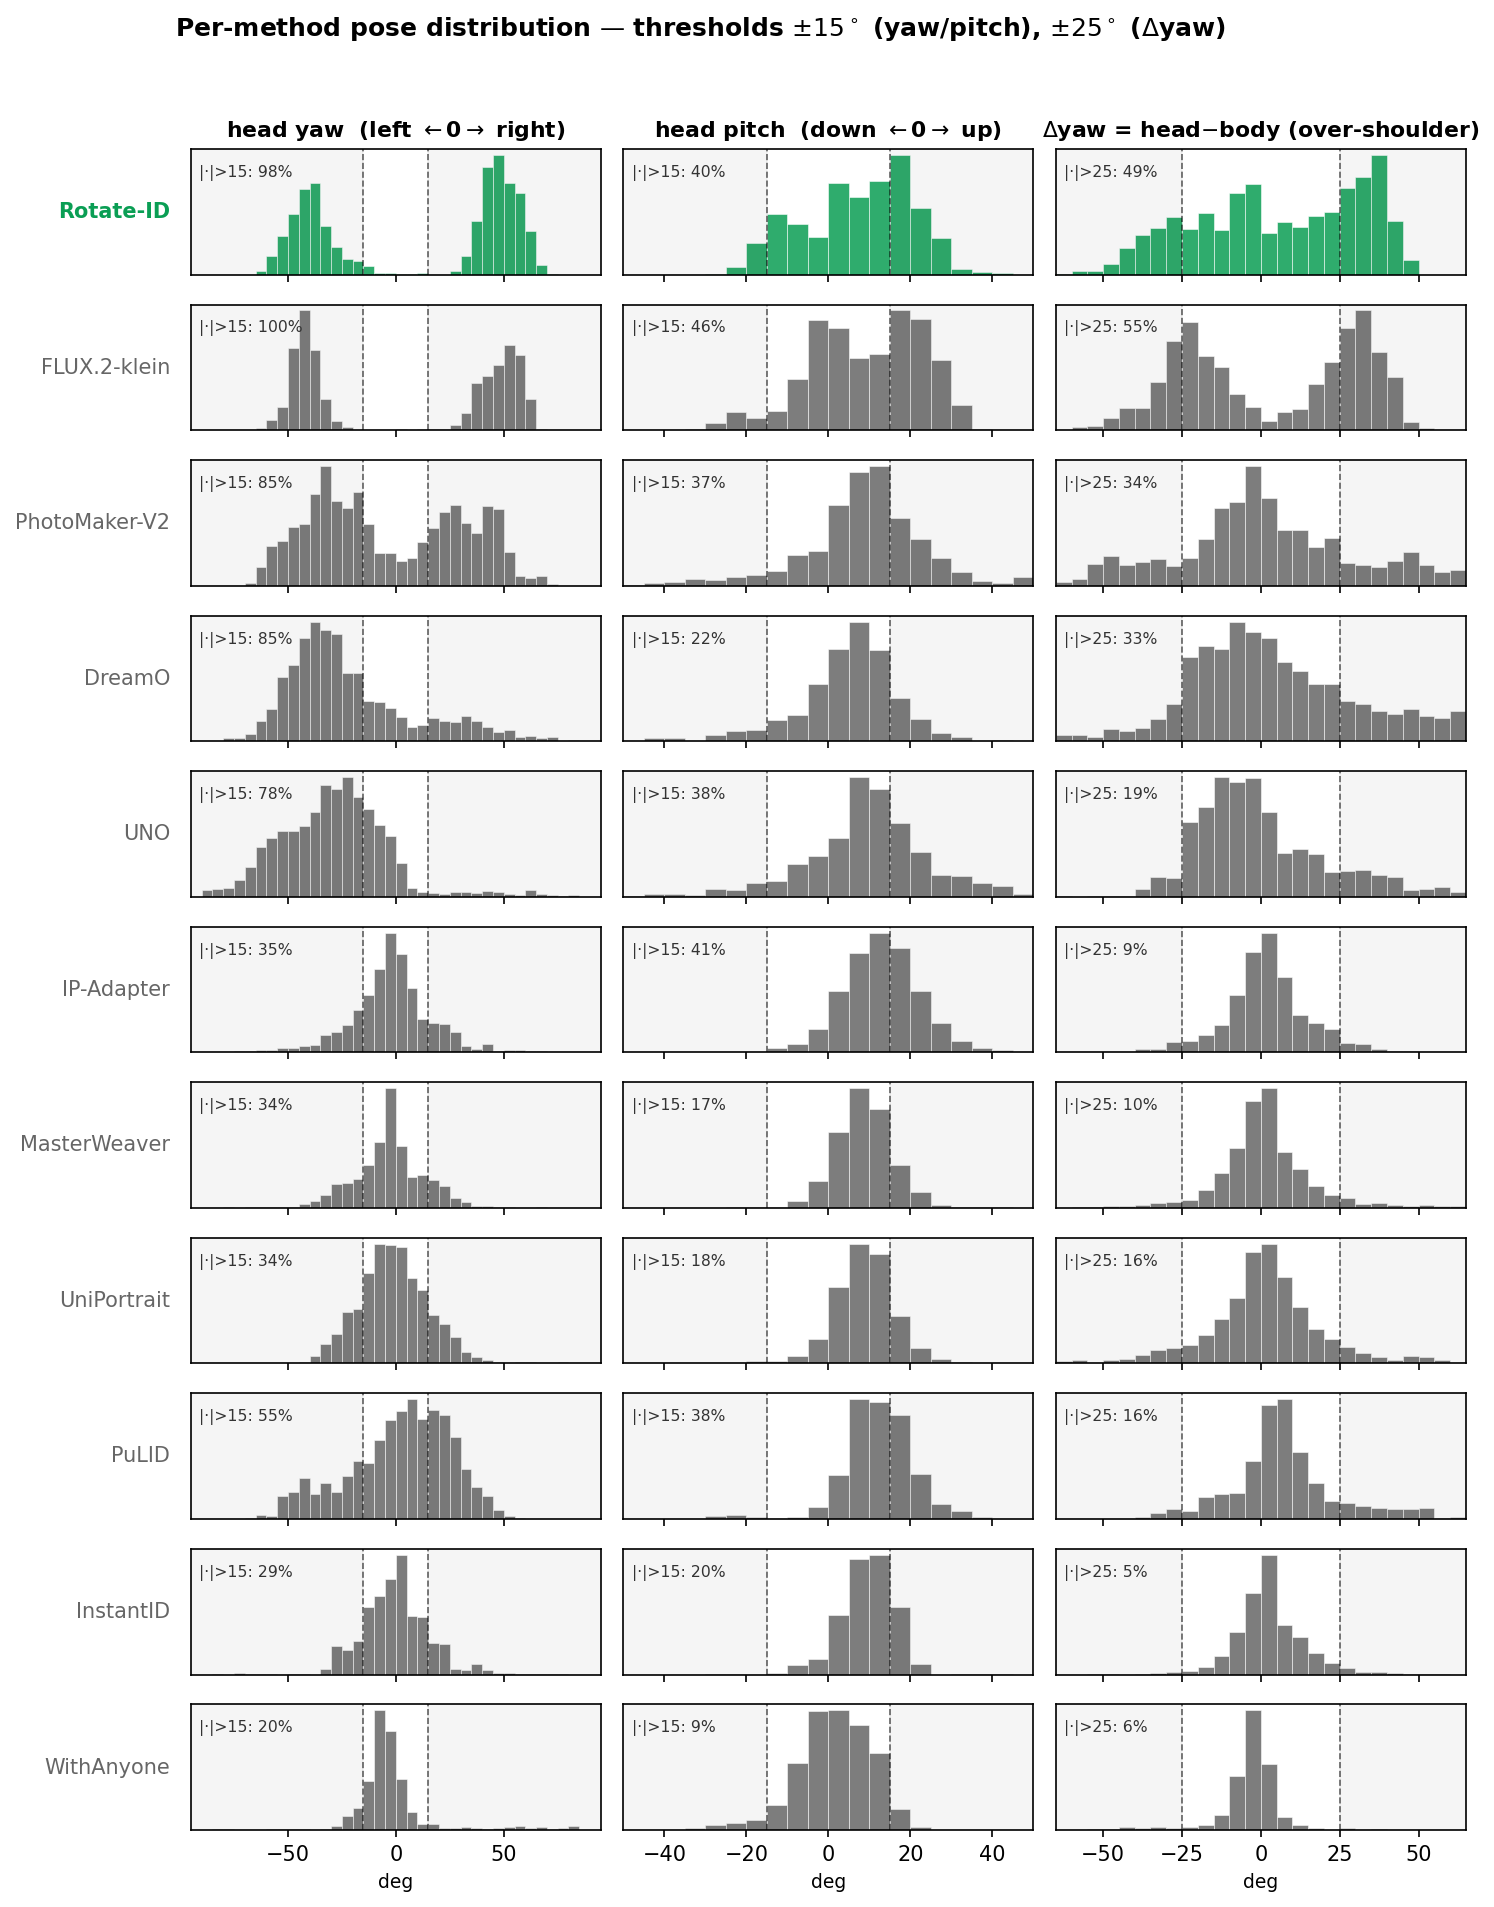
\includegraphics[width=\linewidth]{figures/eval_fig2_method_dist.png}
\caption[Per-method pose distributions]{\textbf{Per-method pose distributions} (head yaw, head pitch, and
$\Delta\theta_y$) with the $\pm15^\circ$ / $\pm25^\circ$ thresholds (dashed) and
hit-zones (shaded), all on the same prompts and estimator. Rotate-ID and the
FLUX.2-klein backbone are \emph{bimodal} in head yaw and $\Delta\theta_y$
(crossing both the turn and over-shoulder lines); the SD adapters collapse inside
$\pm15^\circ$.}
\label{fig:methoddist}
\end{figure}

\section{Robustness of the pose-aware ranking to the yaw/pitch weighting}
\label{sec:appendix_pe}
Our pose-aware identity (Sec.~\ref{sec:metrics}) penalizes by yaw alone,
$P_e{=}1{-}\mathrm{Acc_{yaw}}$, because yaw is the axis our task is defined on. To
confirm the resulting ranking is \emph{not} an artifact of that choice, we
re-evaluate it under the general weighting
$P_e(w){=}w(1{-}\mathrm{Acc_{yaw}})+(1{-}w)(1{-}\mathrm{Acc_{pitch}})$, where
$w{=}1$ recovers the main-text metric and $w{=}\tfrac12$ weights yaw and pitch
\emph{equally}. Table~\ref{tab:pe_robust} reports the pose-aware identity at $k{=}4$
under both. The conclusion is invariant: under \emph{either} weighting,
\textbf{Rotate-ID} is the strongest \emph{tuning-free} method---it overtakes every
tuning-free baseline (equal-weight crossover $k{\approx}1.9$ AdaFace\,/\,$1.5$ PAEs,
vs.\ $1.7/1.0$ for yaw-only)---and the frontal-collapsing baselines' large
\emph{raw} identity lead has evaporated in both. The weighting affects only the
comparison to the per-identity fine-tuned \textbf{DreamBooth}$^\dagger$: under equal
weighting Rotate-ID \emph{ties} it on AdaFace ($0.062$) and leads on PAEs, while
under yaw-only it \emph{surpasses} it---i.e.\ the choice of $w$ changes \emph{how
decisively} Rotate-ID wins, not \emph{whether} it does. The ranking would invert
only as $w{\to}0$ (penalizing pitch alone), a perverse weighting that ignores the
rotation the task asks for; for any $w$ that treats yaw as at least co-equal
($w{\geq}\tfrac12$), Rotate-ID is the best tuning-free method.

\begin{table}[t]\centering\small
\setlength{\tabcolsep}{5pt}
\adjustbox{max width=\linewidth}{%
\begin{tabular}{ll cc @{\hskip 8pt} cc}
\toprule
\multirow{2}{*}{Method} & \multirow{2}{*}{Type} & \multicolumn{2}{c}{equal weight ($w{=}\tfrac12$)} & \multicolumn{2}{c}{yaw-only ($w{=}1$)} \\
\cmidrule(lr){3-4}\cmidrule(lr){5-6}
 & & Ada & PAEs & Ada & PAEs \\
\midrule
\textbf{Rotate-ID (ours)} & ours & \textbf{0.062} & \textbf{0.079} & \textbf{0.148} & \textbf{0.188} \\
\midrule
DreamBooth$^\dagger$~\cite{dreambooth} & fine-tuning & 0.062 & 0.073 & 0.085 & 0.100 \\
\midrule
PhotoMaker-V2~\cite{photomaker} & \multirow{4}{*}{encoder} & 0.030 & 0.034 & 0.035 & 0.039 \\
DreamO~\cite{dreamo} & & 0.031 & 0.034 & 0.040 & 0.044 \\
PuLID~\cite{pulid} & & 0.023 & 0.026 & 0.014 & 0.016 \\
InstantID~\cite{instantid} & & 0.020 & 0.019 & 0.019 & 0.018 \\
\midrule
IP-Adapter~\cite{ipadapter} & adapter & 0.022 & 0.022 & 0.017 & 0.017 \\
\bottomrule
\end{tabular}}
\caption[Robustness of the pose-aware ranking to the yaw/pitch weighting]{\textbf{Robustness of the pose-aware ranking to the yaw/pitch weighting}
(pose-aware identity $\widetilde{\mathrm{CSIM}}$ at $k{=}4$). Under \emph{equal}
weighting ($P_e{=}\tfrac12(1{-}\mathrm{Acc_{yaw}})+\tfrac12(1{-}\mathrm{Acc_{pitch}})$)
and under the main-text \emph{yaw-only} metric ($P_e{=}1{-}\mathrm{Acc_{yaw}}$),
\textbf{Rotate-ID} is the best \emph{tuning-free} method (bold) on both encoders; the
weighting changes only whether it ties or surpasses the per-identity fine-tuned
DreamBooth$^\dagger$.}
\label{tab:pe_robust}
\end{table}

\section{Pose control across backbones: native vs.\ foreign skeleton format}
\label{sec:exp_skel}
A natural question is whether the rotation is merely the backbone: would any
model, given a pose control \emph{in the format it expects}, rotate as well?
Table~\ref{tab:skel} conditions several backbones on a skeleton of the
\emph{same} pose (derived from one shared source render). Two findings. First,
the control \emph{format} matters enormously: a ControlNet fed a foreign SAM-3D
skeleton barely rotates, but the \emph{same} ControlNet fed a detected
\emph{OpenPose} skeleton---its native input---improves sharply (UniPortrait
$22.8\!\rightarrow\!64.6\%$ yaw; SDXL $34.0\!\rightarrow\!52.6\%$). Second, even
with this favorable native control, both ControlNet backbones still trail
Rotate-ID's in-context conditioning on FLUX.2 ($82.6\%$): conditioning through the
joint attention \emph{follows} the target pose more reliably than an external
ControlNet branch.

\noindent\textbf{Takeaway.} \emph{The rotation is not ``any backbone plus a
skeleton'': even with their native control format, ControlNet pipelines trail
in-context conditioning by ${\ge}18$ yaw points.}

\begin{table}[t]\centering\small
\setlength{\tabcolsep}{4pt}
\adjustbox{max width=\linewidth}{%
\begin{tabular}{llccc}
\toprule
Model & Control & Yaw & Pitch & Pose \\
\midrule
\textbf{Rotate-ID} & sam3d (in-context) & \textbf{82.6} & 39.0 & 34.6 \\
UniPortrait & OpenPose (ControlNet) & 64.6 & 43.8 & 22.6 \\
SDXL & OpenPose (ControlNet) & 52.6 & 39.7 & 19.5 \\
\bottomrule
\end{tabular}}
\caption[Following a pose control across backbones]{\textbf{Following a pose control across backbones} (\%; $1400$ images
each). Each ControlNet
backbone is given a detected OpenPose skeleton of the same pose---its \emph{native}
input. Native-format control lifts the ControlNets sharply (cf.\ a foreign SAM-3D
skeleton: UniPortrait $22.8\%$, SDXL $34.0\%$ yaw), yet all trail Rotate-ID's
in-context conditioning.}
\label{tab:skel}
\end{table}

\paragraph{Foreign-format pose control (UniPortrait\,+\,SAM-3D skeleton).}
Table~\ref{tab:skel_appendix} gives the full identity/efficiency breakdown for
UniPortrait conditioned on the \emph{foreign} SAM-3D skeleton---the supplementary
counterpart to the native-OpenPose variant shown above (Table~\ref{tab:skel}).
Feeding the ControlNet a skeleton
outside its training format both lowers face detectability ($74\%$ vs.\ $93\%$,
i.e.\ many more non-detectable faces) and roughly thirds the yaw accuracy
($22.8\%$ vs.\ $64.6\%$). The apparently \emph{higher} aligned identity of the
sam3d variant (Ada$_{\text{det}}$ $0.342$ vs.\ $0.277$) is the same frontal-bias
artifact analysed above: the foreign skeleton barely rotates the head,
so its detected faces sit in the near-frontal regime AdaFace favours. We therefore
promote the native-OpenPose row to the main identity table and keep this
foreign-skeleton variant here for completeness.

\begin{table}[t]\centering\small
\setlength{\tabcolsep}{4.5pt}
\adjustbox{max width=\linewidth}{%
\begin{tabular}{l ccc @{\hskip 8pt} c}
\toprule
Method & Ada$_{\text{det}}$\,$\uparrow$ & PAEs\,$\uparrow$ & Yaw\,$\uparrow$ & \#fail\,$\downarrow$ \\
\midrule
UniPortrait+OpenPose~\cite{uniportrait} & 0.277 & 0.360 & \textbf{64.6} & \textbf{105} \\
UniPortrait+sam3d~\cite{uniportrait}    & 0.342 & 0.406 & 22.8 & 368 \\
\bottomrule
\end{tabular}}
\caption[Pose-conditioned UniPortrait: native vs.\ foreign control]{\textbf{Pose-conditioned UniPortrait: native vs.\ foreign control}
($1400$ generations). The foreign SAM-3D skeleton yields far weaker rotation and
lower detectability than the native OpenPose skeleton; its higher aligned CSIM is
the frontal-bias artifact (it barely turns). The OpenPose row (also in
Table~\ref{tab:skel}) is the one promoted to the main results.}
\label{tab:skel_appendix}
\end{table}

\section{Backbone choice: rotation quality and resource efficiency}
\label{sec:appendix_backbone}
\paragraph{Text-driven rotation across T2I backbones.}
Before adding any structural control, we compare six T2I backbones at text-driven
head rotation on the balanced 40-prompt benchmark (Sec.~\ref{sec:exp_setup}),
justifying the FLUX.2-klein base used throughout (Sec.~\ref{sec:pose}).
FLUX.2-klein attains the best yaw accuracy, motivating it as our base
(Table~\ref{tab:backbone}). The other backbones trail it: while autoregressive
models like Janus-Pro reach competitive geometric retention ($45\%$ yaw) from
large-scale joint pretraining, they still lack the decoupled spatial control
needed for the extreme-profile regime---only $1/40$ of Janus's generations reach
$|\theta_y|{\geq}60^\circ$. This establishes that the ceiling for text-only
rotation is already highest here, before any structural control---which is why the
explicit pose control of Sec.~\ref{sec:pose} is needed to realize profile views
reliably.

\begin{table}[t]\centering\small
\setlength{\tabcolsep}{5pt}
\adjustbox{max width=\linewidth}{%
\begin{tabular}{lccc}
\toprule
Backbone & Yaw acc & Pitch acc & mean\,$|\theta_y|$ \\
\midrule
\textbf{FLUX.2-klein} (base) & \textbf{67.5} & 40.0 & 50.4 \\
Sana~\cite{sana} & 55.0 & 42.5 & 53.7 \\
Janus-Pro-7B~\cite{janus} & 45.0 & 27.5 & 35.7 \\
SoftREPA (SD3)~\cite{softrepa} & 42.5 & 37.5 & 59.6 \\
Infinity~\cite{infinity} & 35.0 & 37.5 & 30.2 \\
HART~\cite{hart} & 32.5 & 42.5 & 38.2 \\
\bottomrule
\end{tabular}}
\caption[Text-driven head rotation across six T2I backbones]{\textbf{Text-driven head rotation across six T2I backbones} ($40$ pose
prompts, one image each; accuracy in \%, $|\theta_y|$ in degrees). FLUX.2-klein
attains the best yaw accuracy while turning the head substantially; the remaining
backbones trail it---the autoregressive Janus-Pro rotates ($45\%$ yaw) from
large-scale pretraining but rarely reaches extreme profile ($1/40$ at
$|\theta_y|{\geq}60^\circ$). We adopt FLUX.2-klein as the base backbone.}
\label{tab:backbone}
\end{table}

\paragraph{Resource efficiency: why a 4B backbone.}
\label{sec:exp_resource}
A practical constraint shapes the backbone choice: the differentiable gate training
and the $1400$-generation benchmark must run on a single $32$\,GB card, which rules
out the $20$B-class instruction editors. Qwen-Image-Edit-2511's $28.8$\,B parameters
($20.4$\,B MM-DiT $+$ $8.3$\,B vision-language encoder) need $57.7$\,GB in bf16,
\emph{exceeding} the card, so it cannot run un-quantized on one GPU; even at $4$-bit
(GGUF-Q4) with a $4$-step Lightning distillation and CPU offload---the fastest
configuration that fits---it generates at only ${\sim}79$\,s/img (${\sim}250$\,s for
the first, warm-up image). FLUX.2-klein ($4$\,B, ${\sim}8$\,GB
weights) fits comfortably and generates an order of magnitude faster
(Table~\ref{tab:resource}), leaving the headroom the gate training needs---while
the two editors we do run at full scale, Step1X-Edit and OmniGen2, neither
rotate reliably nor preserve identity
(Tables~\ref{tab:sota_pose},~\ref{tab:posepenalized}). Peak VRAM and latency are
measured with a warm-up phase and \texttt{torch.cuda.max\_memory\_allocated}.

\begin{table}[t]\centering\small
\setlength{\tabcolsep}{5pt}
\adjustbox{max width=\linewidth}{%
\begin{tabular}{lccc}
\toprule
Model & Params & bf16 weights & s/img \\
\midrule
\textbf{Rotate-ID} (FLUX.2-klein) & $4$\,B & ${\sim}8$\,GB & $6.5$--$10.1$ \\
Qwen-Image-Edit-2511~\cite{qwenimageedit} & $28.8$\,B & $57.7$\,GB$^\dagger$ & ${\sim}79^\ddagger$ \\
Step1X-Edit~\cite{step1xedit} & $20.8$\,B & $41.6$\,GB$^\dagger$ & $13.1$ \\
OmniGen2~\cite{omnigen2} & $7.8$\,B & $15.6$\,GB & $9.0$ \\
\bottomrule
\end{tabular}}
\caption[Backbone resource efficiency]{\textbf{Backbone resource efficiency.} bf16 weight footprint and
steady-state $1024^2$ generation time on one RTX~5090 ($32$\,GB).
$^\dagger$exceeds the card, so bf16 inference OOMs on a single GPU (requires
quantization or CPU offload; Step1X-Edit is run with an FP8 transformer);
$^\ddagger$GGUF-Q4 $+$ $4$-step Lightning $+$ CPU offload (the only config that
fits; bf16 and fp8 OOM). Parameter counts are measured from the released weights
(Step1X-Edit: $12.4$\,B DiT $+$ $8.3$\,B Qwen2.5-VL encoder; OmniGen2: $4.0$\,B
DiT $+$ $3.8$\,B Qwen2.5-VL MLLM). The $4$B FLUX.2-klein is an order of magnitude
faster and is the only option leaving headroom for the differentiable gate
training; the editors' s/img is from Table~\ref{tab:sota_pose}.}
\label{tab:resource}
\end{table}

\section{Verifying the reference-conditioning pathway: full data}
\label{sec:appendix_causal}
Sec.~\ref{sec:refverify} argued causally that identity survives FLUX.2-klein's
in-context conditioning through three verified links: the VAE preserves
identity-relevant detail, the raw pre-attention reference tokens do not yet
encode it legibly, and the transformer's joint attention reads it from the
reference's \emph{content} rather than its sequence position. We give the
complete data for each here.

\paragraph{(i) VAE round-trip.} We encode-then-decode $34$ reference identities
through the frozen VAE alone (no denoising, no transformer) and score AdaFace
and PAEs cosine between each original $I_{\mathrm{id}}$ and its reconstruction
$I_{\mathrm{id}}^{\mathrm{recon}}$, against a same-set impostor baseline
(Table~\ref{tab:vaeroundtrip}, Fig.~\ref{fig:vaeroundtrip}). Reconstruction
pairs separate from impostor pairs by $+0.96$ AdaFace / $+0.83$ PAEs cosine;
the one reconstruction without a detectable face (Yayoi, dropped from the
table) fails at \emph{face detection}, not identity, and the lowest-scoring
detected pair (Jane, $0.82$) still sits far above the impostor ceiling
($0.20$). The codec is not where identity would be lost.

\begin{table}[t]\centering\small
\setlength{\tabcolsep}{5pt}
\adjustbox{max width=\linewidth}{%
\begin{tabular}{lc cc}
\toprule
Comparison & $n$ & AdaFace CSIM & PAEs CSIM \\
\midrule
Reconstruction ($I_{\mathrm{id}}$ vs.\ recon.) & $33$ & $0.961\pm0.037$ & $0.873\pm0.127$ \\
Impostor ($I_{\mathrm{id},i}$ vs.\ $I_{\mathrm{id},j}$) & $1122$ & $0.005\pm0.055$ & $0.044\pm0.096$ \\
\bottomrule
\end{tabular}}
\caption[VAE round-trip identity preservation]{\textbf{VAE round-trip identity preservation} (mean$\pm$std cosine).
Reconstruction pairs (same identity, before vs.\ after the frozen VAE encode-decode)
separate from same-set impostor pairs (different identities, both originals) by
$+0.956$ AdaFace / $+0.830$ PAEs---the VAE alone does not discard
identity-discriminative detail.}
\label{tab:vaeroundtrip}
\end{table}

\begin{figure}[t]\centering
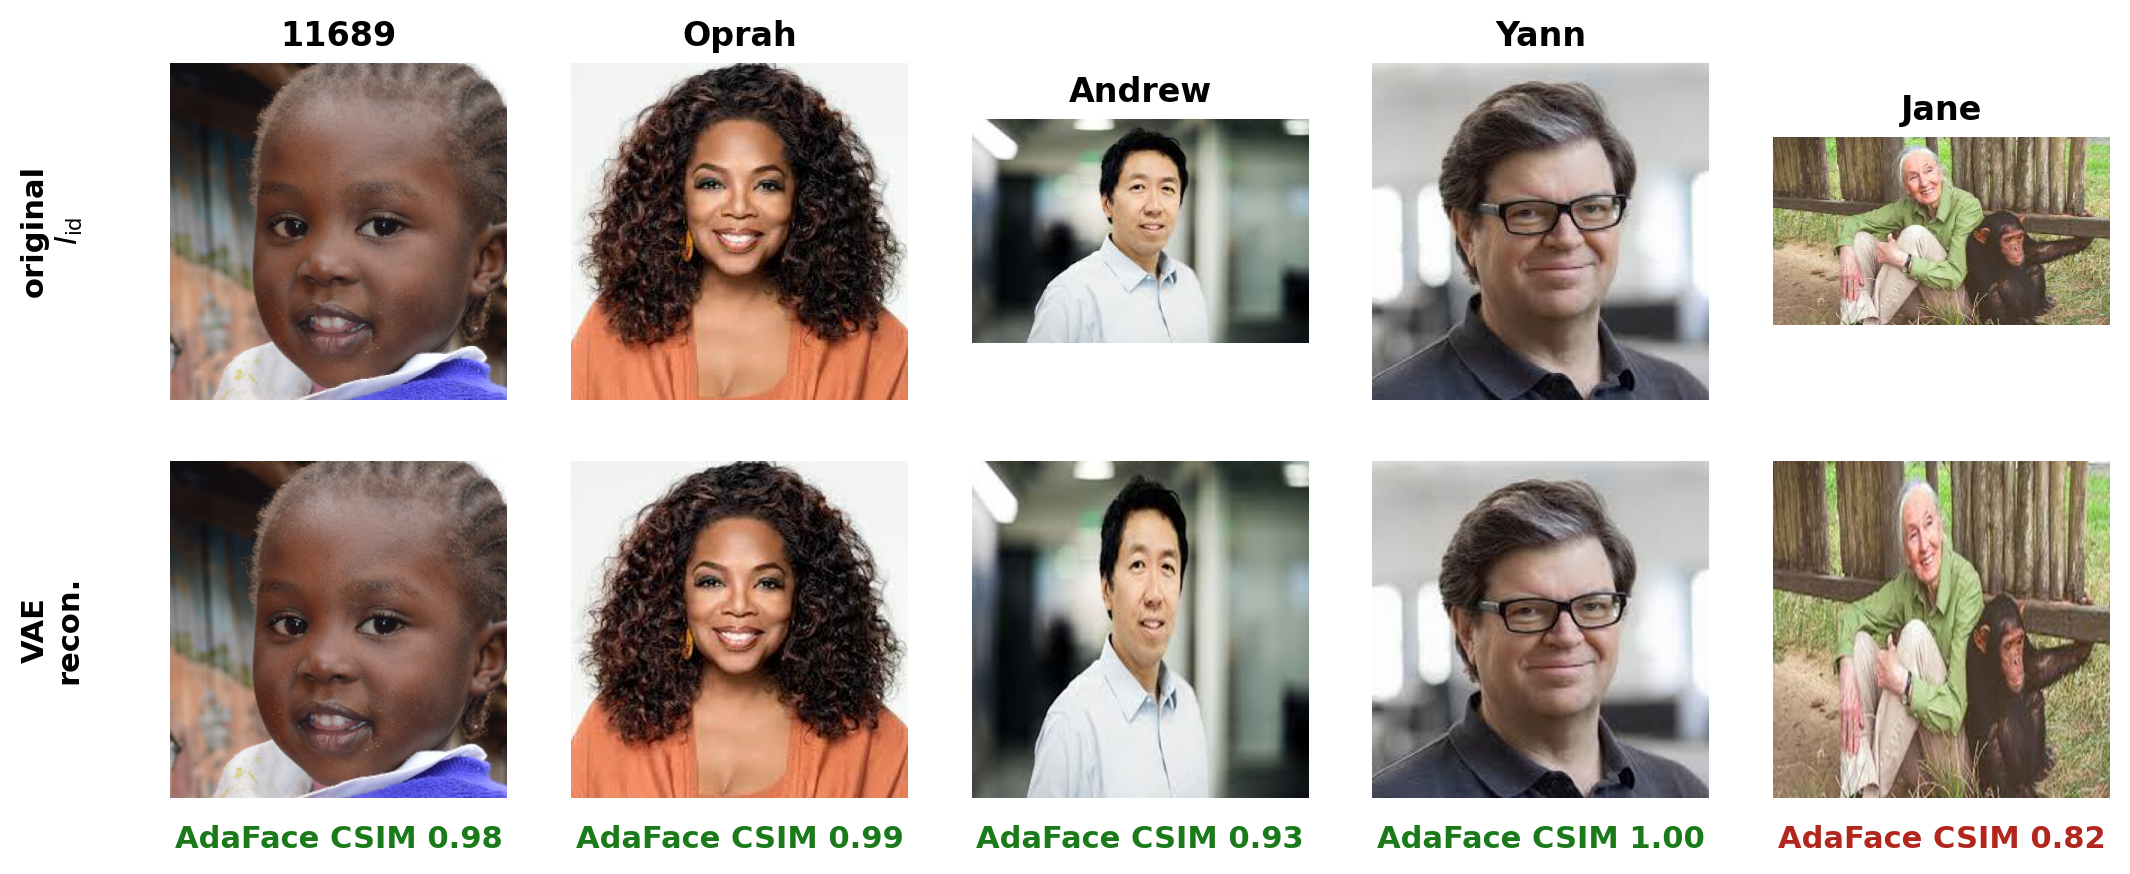
\includegraphics[width=\textwidth]{figures/causal_vae_roundtrip.png}
\caption[VAE round-trip qualitative]{\textbf{VAE round-trip qualitative} (Table~\ref{tab:vaeroundtrip}).
Five identities, original (top) vs.\ frozen-VAE reconstruction (bottom; no
transformer, no denoising), with AdaFace cosine to the original below each.
Reconstructions are visually near-identical to their originals across skin
tone, age, and accessories; even the weakest case in the set (Jane, $0.82$)
is far above the $0.20$ impostor ceiling.}
\label{fig:vaeroundtrip}
\end{figure}

\paragraph{(ii) Reference-token geometry.} Before any attention runs, we pool the
patch-embedded, pre-RoPE identity tokens $C_{\mathrm{id}}$---by face region, by
whole image, and by background---for the $35$ identities and test their
correspondence to the AdaFace embedding space: representational similarity
(Spearman $\rho$ between the FLUX-token and AdaFace pairwise-cosine matrices)
and top-1 nearest-neighbor agreement, against a skeleton-token null control
(Table~\ref{tab:tokengeometry}). Every pooling, \emph{including the face
region}, is statistically indistinguishable from the null control and from
chance agreement. We report this as a genuine null result: raw reference
tokens are not already a face embedding, so whatever identity structure the
model uses is not linearly present before attention---it must be extracted by
the transformer itself, consistent with (iii) below and with the
attention-budget account of Sec.~\ref{sec:mechanism}.

\begin{table}[t]\centering\small
\setlength{\tabcolsep}{5pt}
\adjustbox{max width=\linewidth}{%
\begin{tabular}{lcc}
\toprule
Pooling of $C_{\mathrm{id}}$ ($n{=}35$) & RSA $\rho$ ($p$) & top-1 agree.\ (chance) \\
\midrule
face-region & $+0.021$ ($0.61$) & $0.029$ ($0.029$) \\
whole image & $+0.044$ ($0.28$) & $0.029$ ($0.029$) \\
background & $+0.051$ ($0.22$) & $0.057$ ($0.029$) \\
\midrule
skeleton $C_S$ (null control) & $-0.029$ ($0.49$) & $0.029$ ($0.029$) \\
\bottomrule
\end{tabular}}
\caption[Pre-attention reference-token geometry vs.\ AdaFace]{\textbf{Pre-attention reference-token geometry vs.\ AdaFace} (null
result). None of the poolings---including the face region---correlate with the
AdaFace similarity structure above the skeleton null control or chance
nearest-neighbor agreement. Identity is not yet legible in the raw, pre-RoPE
patch embedding; see (iii) for where it is causally used.}
\label{tab:tokengeometry}
\end{table}

\paragraph{(iii) Content-vs-position causal swap.} Holding prompt, skeleton,
seed, and the trained \gate{} fixed, we vary only the pixels occupying the
identity slot across four conditions for $10$ identity pairs $(A,B)$---the real
photo of $A$ (\emph{normal-$A$}), a swap to $B$ (\emph{swap-$B$}), a
content-free grey block (\emph{blank-ID}), and $A$ with the face region masked
out (\emph{face-masked-$A$})---and score every output against both $A$'s and
$B$'s original photos (Table~\ref{tab:causalswap}, Fig.~\ref{fig:causalswap}).
Output identity tracks the swap: CSIM-to-$A$ is $0.34$ under the real photo and
falls to $\leq\!0.02$ under \emph{every} content ablation, while CSIM-to-$B$
rises to $0.28$ exactly when $B$'s photo---not $A$'s---occupies the identical
slot. Masking only the face region collapses identity as completely as a blank
block, so the effect is specifically the \emph{face content}, not merely "a
reference image is present." The slot position is identical across all four
conditions, so position alone cannot explain any of this variation.

\begin{table}[t]\centering\small
\setlength{\tabcolsep}{5pt}
\adjustbox{max width=\linewidth}{%
\begin{tabular}{lc c cc}
\toprule
Condition & $n$ & face det.\ & CSIM-to-$A$ & CSIM-to-$B$ \\
\midrule
normal-$A$ & $10$ & $8/10$ & $\mathbf{0.341}$ & $0.015$ \\
swap-$B$ & $10$ & $7/10$ & $-0.014$ & $\mathbf{0.280}$ \\
blank-ID & $10$ & $7/10$ & $-0.023$ & $-0.006$ \\
face-masked-$A$ & $10$ & $8/10$ & $-0.000$ & $-0.010$ \\
\bottomrule
\end{tabular}}
\caption[Content-vs-position causal swap]{\textbf{Content-vs-position causal swap} (mean AdaFace cosine over
detected faces; identical prompt/skeleton/seed/\gate{} across all four
conditions, only the identity-slot pixels vary). Identity follows reference
\emph{content}: CSIM-to-$A$ is high only under \emph{normal-$A$}, CSIM-to-$B$
is high only under \emph{swap-$B$}, and both collapse under \emph{blank-ID}
and \emph{face-masked-$A$}---ruling out slot position as the explanation.}
\label{tab:causalswap}
\end{table}

\begin{figure}[t]\centering
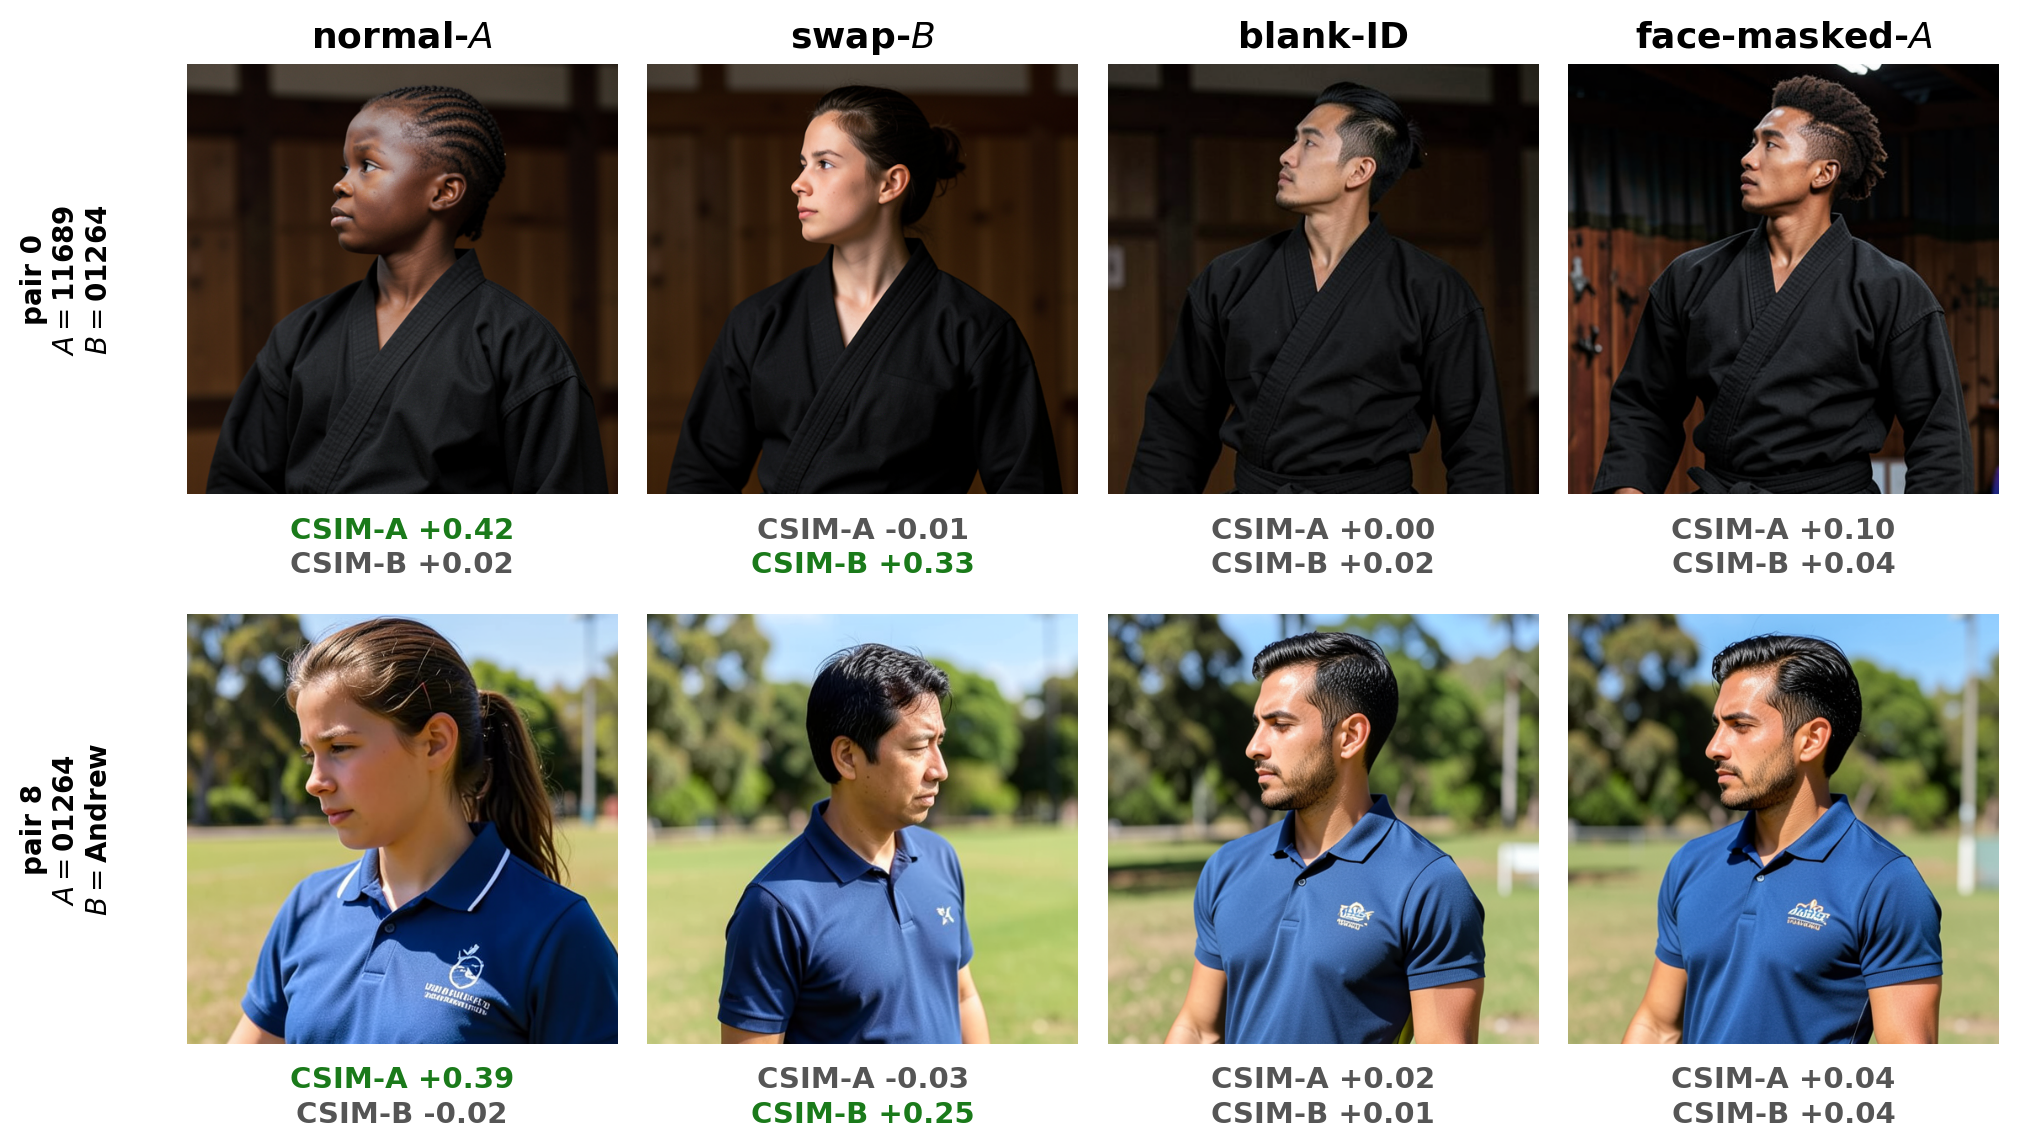
\includegraphics[width=\textwidth]{figures/causal_swap_grid.png}
\caption[Content-vs-position causal swap, qualitative]{\textbf{Content-vs-position causal swap, qualitative} (Table~\ref{tab:causalswap}).
Two pairs (rows), four conditions (columns), identical prompt/skeleton/seed/\gate{}
within a row---only the identity-slot content changes. \emph{normal-$A$} renders
$A$; \emph{swap-$B$} renders $B$ in the same slot, same pose, same scene;
\emph{blank-ID} and \emph{face-masked-$A$} both collapse to a generic person
resembling neither reference. CSIM-to-$A$/$B$ annotated below each image (green:
the reference actually used).}
\label{fig:causalswap}
\end{figure}

\section{Reference order: the earlier block wins the budget}
\label{sec:appendix_ordering}
Sec.~\ref{sec:refgeometry} predicts that \emph{order} is a real variable: the
first-listed reference sits closest to the generation on the RoPE $t$-axis
(Eq.~\ref{eq:ropeids}) and should receive more attention. We verify this at
generation scale with a controlled swap---identical prompts, seed, duplication,
and learned gate; \emph{only} the list order changes from
$[C_{\mathrm{id}}{\times}3,\,C_S]$ to $[C_S,\,C_{\mathrm{id}}{\times}3]$
(Fig.~\ref{fig:ordering}). Placing the skeleton first costs $0.070$ AdaFace
($0.392\!\rightarrow\!0.322$) and $0.033$ pose-aware identity
($0.168\!\rightarrow\!0.135$) at \emph{unchanged} yaw
($78.8\%$ vs.\ $78.2\%$)---order is a pure identity lever. The attention probe
of Sec.~\ref{sec:mechanism} agrees: the measured identity share drops from $0.121$ (id-first) to $0.103$
(skeleton-first), while pose is insensitive because the skeleton's geometry is
absorbed in the early structure-setting steps regardless of position. Together
with the duplication sweep (Sec.~\ref{sec:exp_ablate}), this closes the loop on
Sec.~\ref{sec:refgeometry}: both training-free levers act exactly as the
token-geometry account predicts.

\begin{figure}[t]\centering
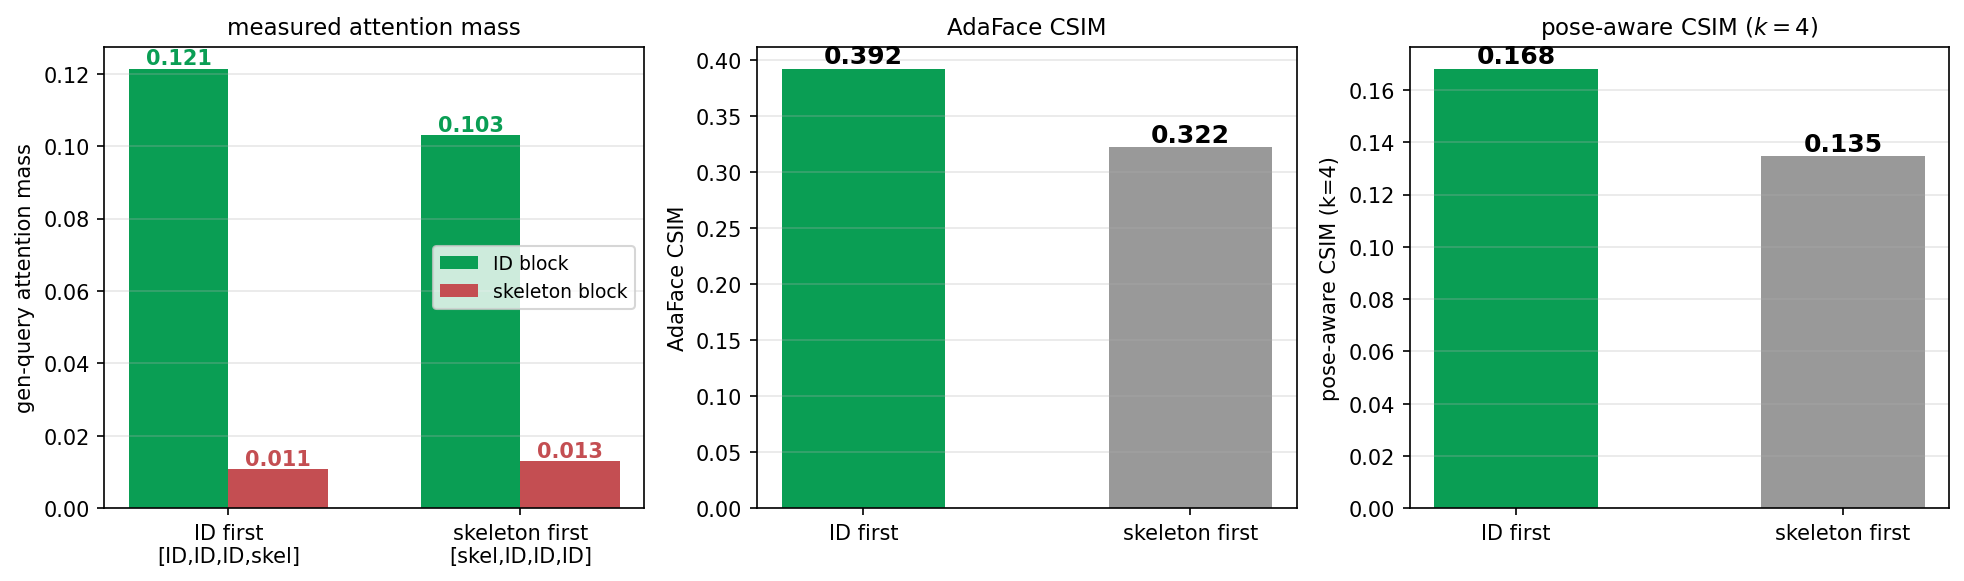
\includegraphics[width=\linewidth]{figures/mech_ordering_summary.png}
\caption[Ordering ablation]{\textbf{Ordering ablation} (identical prompts/seed/duplication/gate;
only the reference list order differs). Left: measured gen-query attention mass
(probe)---the earlier position receives $+18\%$ identity mass. Middle/right:
AdaFace and pose-aware identity on the same $170$-pair grid; yaw is unchanged
($78.8\%$ vs.\ $78.2\%$), so order is a pure identity lever, as the RoPE
$t$-coordinate geometry (Eq.~\ref{eq:ropeids}) predicts.}
\label{fig:ordering}
\end{figure}

\section{Pose-angle extraction: exact formulas}
\label{sec:appendix_angles}
This section gives the full geometry summarized in Sec.~\ref{sec:metrics}.
\emph{Head yaw} $\theta_y$ and \emph{head pitch} $\theta_p$ come from the head's
global rotation $R_{\mathrm{head}}$, formed by composing the SMPL-X forward
kinematics along the spine chain
(pelvis$\to$spine1$\to$spine2$\to$spine3$\to$neck$\to$head) and calibrating
against the upright reference $R_{\mathrm{up}}{=}R_x(\pi)$: $\theta_y$ is the
Euler-$y$ component of $R_{\mathrm{up}}^{-1}R_{\mathrm{head}}$, while---to avoid
Euler gimbal lock at large yaw---$\theta_p$ is read from the head forward axis
$f$ (third column of $R_{\mathrm{head}}$) as its elevation above the horizontal,
$\theta_p=\operatorname{atan2}\!\big(f_y,\sqrt{f_x^2+f_z^2}\big)$, plus a fixed
$19^\circ$ anatomical offset that re-centers SMPL-X's rest head pose to level
gaze. The \emph{head-to-torso yaw} $\Delta\theta_y$ is \emph{not} an Euler
difference but a 3D-geometry angle between two unit forward normals: a head
normal
$n_{\mathrm{h}}\propto(p_{\text{r-ear}}{-}p_{\text{l-ear}})\times(p_{\text{nose}}{-}\bar p_{\mathrm{h}})$,
$\bar p_{\mathrm{h}}{=}\mathrm{mean}(p_{\text{nose}},p_{\text{l-eye}},p_{\text{r-eye}})$,
and a torso normal
$n_{\mathrm{b}}\propto(p_{\text{r-sh}}{-}p_{\text{l-sh}})\times(p_{\text{neck}}{-}\bar p_{\mathrm{b}})$,
$\bar p_{\mathrm{b}}{=}\mathrm{mean}(p_{\text{neck}},p_{\text{l-sh}},p_{\text{r-sh}})$;
$\Delta\theta_y$ is the signed yaw between their horizontal ($x$--$z$)
projections, $\operatorname{atan2}(\det,\mathrm{dot})$, canonicalized to a
consistent branch. $|\Delta\theta_y|$ is large exactly when the head is turned
far relative to the chest.

\section{Reading identity at profile: the full evidence}
\label{sec:appendix_profile}

\paragraph{What the PAEs are.} \textbf{Pose-Adapted face Encoders (PAEs)} are a
bank of six pose-specialized recognizers
$\{E_{ff},E_{ss},E_{pp},E_{fs},E_{sp},E_{fp}\}$ from PASL~\cite{pasl}, each
adapted to a pair of yaw regimes (frontal $<\!30^\circ$, side
$30\text{--}60^\circ$, profile $\geq\!60^\circ$). Each generated/reference pair
is routed to the encoder matching its two \emph{measured} yaw bins---these
regimes exist only for routing, never as requested categories---and that
encoder's cosine is reported. PAEs thus measure the identity that
\emph{survives} rotation rather than identity as seen by a frontal-only
encoder; because the bank sits outside the generator, the read-out is a
drop-in tool for any task that must preserve identity under large
out-of-plane pose.

Section~\ref{sec:identity} claims the frontal-to-profile \csim{} drop is largely
a recognizer artifact; three pieces of evidence separate the artifact from a
real identity loss. \textbf{(i)~Pose-adapted recovery.} The pose-robust PAEs
read-out recovers much of the apparent profile loss---the angle-matched encoder
still finds the identity (Table~\ref{tab:sota_pose}).
\textbf{(ii)~Cross-encoder agreement.} Three pose-adapted recognizers---the
bin-routed PAEs and the single cross-pose experts $E_{fs}$ and $E_{fp}$ applied
to every image, all ArcFace-family encoders distinct from AdaFace---agree to
within $\sim\!0.04$ on every method and read consistently above the frontal
AdaFace cosine on the methods that rotate (Rotate-ID $0.38$ vs.\ $0.30$), so the
recovered identity reproduces across recognizers rather than being one encoder's
fluke. \textbf{(iii)~An irreducible floor.} Even between two \emph{real}
photographs of the same person, automatic verifiers lose roughly ten cosine
points from frontal to profile (the CFP gap~\cite{cfp}), so part of the profile
decrease \emph{every} method exhibits is a property of recognition itself, not a
generation failure. Crucially, the comparison conditions identity on
\emph{having achieved the pose}: a personalizer that collapses to frontal is
never tested at profile, so we read identity only over images that actually
rotated.
